\documentclass{resume}

\begin{document}

\fontfamily{ppl}\selectfont

\noindent
\begin{tabularx}{\linewidth}{@{}m{0.8\textwidth} m{0.2\textwidth}@{}}
{
    \Large{Rubén Tobar Nicolau} \newline
    \small{
        \clink{
            \href{mailto:rubentobarnicolau@gmail.com}{rubentobarnicolau@gmail.com} 
            \textbf{·} 
            {\fontdimen2\font=0.75ex 677 11 91 39}
%            \textbf{·}
%            \href{https://www.rubtobar.com}{rubtobar.com}
            
            \href{https://www.linkedin.com/in/rubtobar/}{linkedin.com/in/rubtobar/}
            \textbf{·} 
    		\href{https://github.com/rubtobar}{github.com/rubtobar}
    	} \newline
        Madrid, Spain
    }
} & 
{
    \hfill
    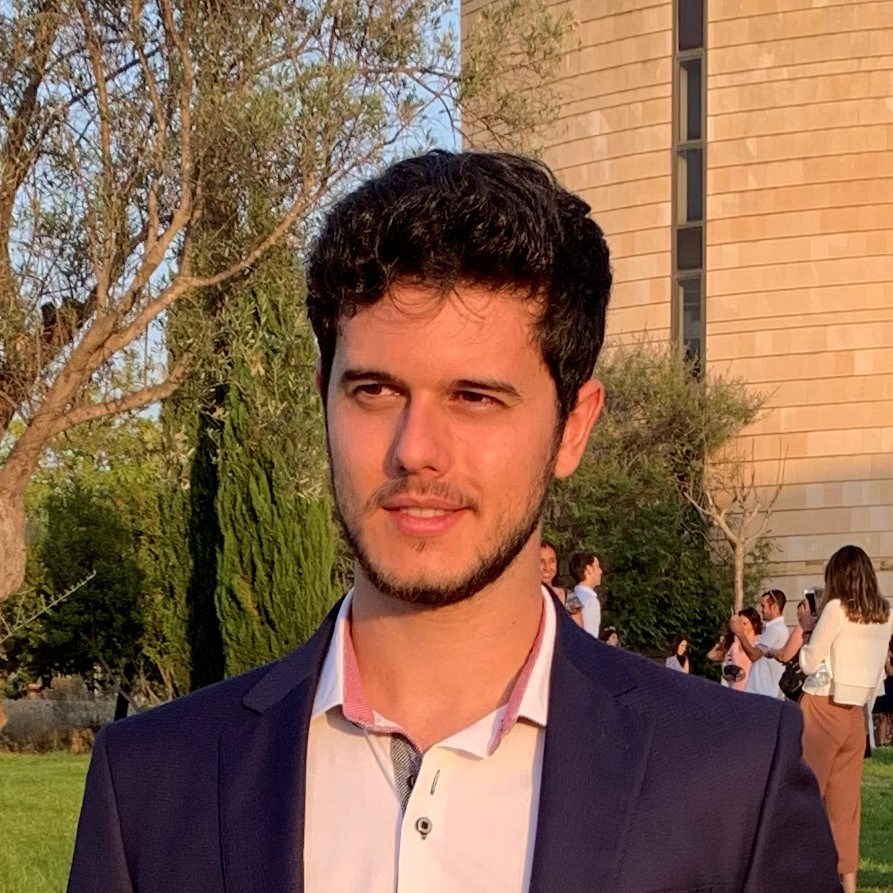
\includegraphics[width=2.8cm]{images/me.jpg}
}
\end{tabularx}

\begin{center}
\begin{tabularx}{\linewidth}{@{}*{2}{X}@{}}
% left side %
{
    \csection{Experience}{\small
        \begin{itemize}
            % item 1 %
			\item 
			\textbf{ISDEFE} \newline
			Systems and Cybersecurity engineer
			\begin{itemize}
				\item System Administration
				\item Cybersecurity
				\item Data mining
				\item Continuous training
			\end{itemize}
			\begin{footnotesize}
			\textit{March 2020 - Current}
			\end{footnotesize}
			
            % item 2 %
            \item 
            \textbf{Juniper Innovating Travel Technology} \newline
            Software engineer
            \begin{itemize}
            	\item Company with global reach
            	\item Software requirements elicitation
            	\item .NET framework
            	\item Booking engine
            \end{itemize}
            \begin{footnotesize}
            	\textit July 2017 - October 2017
            \end{footnotesize}
            
            
        \end{itemize}
    
    }
    \csection{Formación}{\small
        \begin{itemize}
            % item 1 %
            \item \frcontent{Master's Degree in Artificial Intelligence}{International University of La Rioja}{}{Ongoing}
            % item 2 %
            \item \frcontent{Degree in Computer Engineering}{University of the Balearic Islands}{}{2019}
            % item 3 %
            \item \frcontent{ERASMUS+ in Bologna, Italy}{Alma Mater Studiorum Università di Bologna}{}{2017}
        \end{itemize}
    }
    \csection{Other information}{\small
        \begin{itemize}
        	% item 1 %
        	\item \textbf{Languages} \newline Spanish y Catalan (Native), English (High)
        	\footnotesize
        \end{itemize}
    }
} 
% end left side %
& 
% right side %
{
    \csection{Tecnologies}{\small
        \begin{AutoMultiColItemize}
			\item Java
			\item Python
			\item C++
			\item C\#
			\item C
			\item JavaScript
			\item TensorFlow
			\item Kubernetes
			\item Angular
			\item Flutter
			\item Dockers
			\item .NET
			\item Bash
        \end{AutoMultiColItemize}
    }
    \csection{Projects}{\small
        \begin{itemize}
            \item \frcontent{Compiler \newline \clink{
            		\href
            		{https://github.com/rubtobar/compiler}
            		{\footnotesize [github.com/rubtobar/compiler]}}}
            	{Compiler from java-like language to assembly code.}{}{Java, Assebly Code, Regex, LARL Parser Generator.}
            \item \frcontent{Morphologic Filters \newline \clink{
            		\href{https://github.com/rubtobar/filtros-morfologicos}
            		{\footnotesize[github.com/rubtobar/filtros-morfologicos]}}}
            	{Remove impulsive noise in binary fingerprint images.}{}{Python, Jupyter Notebook, OpenCV}
            \item \frcontent{Model View Controller \newline 
            \clink{
            	\href{https://github.com/rubtobar/MVC}
            	{\footnotesize[github.com/rubtobar/MVC]}}}
            {Hotel reservation management system using relational database, MVC and Razor.}{}{C\#, .NET 5.0, Razor, SQL Database}
            \item \frcontent{File system \newline 
            \clink{
            	\href{https://github.com/rubtobar/file-system}
            	{\footnotesize[github.com/rubtobar/file-system]}}}
        {File system with implemented MUTEX semaphores for concurrency.}{}{C, Make, Linux, Shell}
        \end{itemize}
    }
    \csection{Interests \& Hobbies }{\small
        \vspace{0.32cm}
        \begin{tabularx}{\linewidth}{@{}*{4}{>{\centering\arraybackslash}X}@{}}
            {\centering
            
\includegraphics[width=0.8cm]{images/sports.png}
            } &
            {\centering
            
\includegraphics[width=0.8cm]{images/camera.png}
            } & 
            {\centering
            
\includegraphics[width=0.8cm]{images/guitar.png}
            } &
            {\centering
            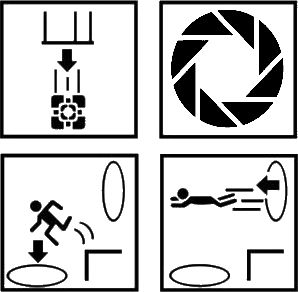
\includegraphics[width=0.8cm]{images/aperture.png}
            } \\
            {\footnotesize Sports} & {\footnotesize Photography} & {\footnotesize Gitar} & {\footnotesize New Technologies}
        \end{tabularx}
    }
}
\end{tabularx}
\end{center}
\end{document}